%\documentclass[tikz,convert={density=800,outext=.png},border=5pt]{standalone}
\documentclass[preview]{standalone}

\usepackage[utf8]{inputenc} % utf8 encoding

\usepackage{tikz}
\usetikzlibrary{positioning}

\begin{document}

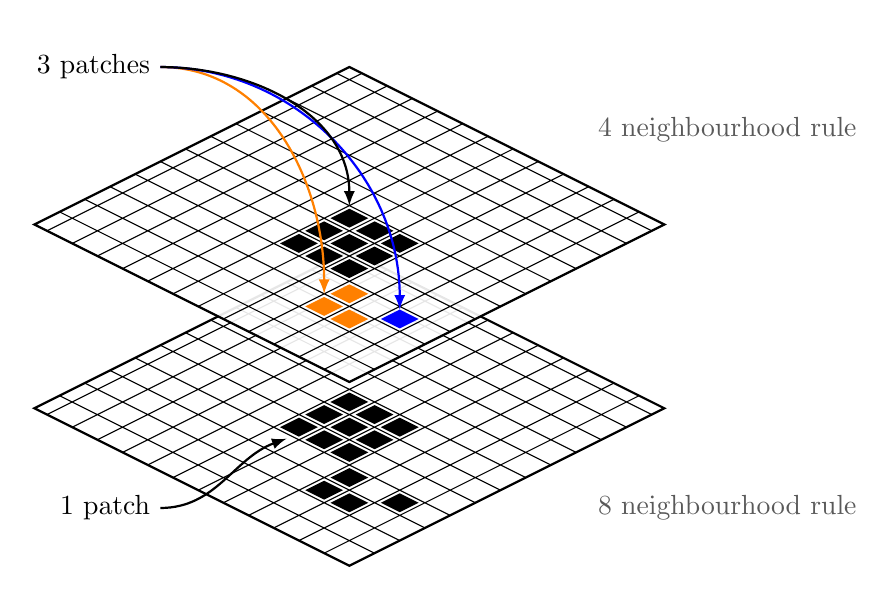
\begin{tikzpicture}[scale=.8,every node/.style={minimum size=1cm},on grid]
%
   \begin{scope}[
           yshift=-83,every node/.append style={
           yslant=0.5,xslant=-1},yslant=0.5,xslant=-1
           ]
       \draw[step=4mm, black] (0,0) grid (5,5);
       \draw[black,thick] (0,0) rectangle (5,5);%borders
       \fill[black] (2.05,2.05) rectangle (2.35,2.35); % center pixel
       \fill[black] (1.65,2.05) rectangle (1.95,2.35); %left
       \fill[black] (2.45,2.05) rectangle (2.75,2.35); %right
       \fill[black] (2.05,2.45) rectangle (2.35,2.75); %top
       \fill[black] (2.05,1.95) rectangle (2.35,1.65); %bottom
% 8 -pixel setting
       \fill[black] (1.65,2.45) rectangle (1.95,2.75); %top-left
       \fill[black] (2.45,2.45) rectangle (2.75,2.75); %top-right
       \fill[black] (2.75,1.95) rectangle (2.45,1.65); %bottom-right
       \fill[black] (1.65,1.95) rectangle (1.95,1.65); %bottom-left
% 2. ring
       \fill[black] (1.25,1.55) rectangle (1.55,1.25); %bottom-left
       \fill[black] (0.85,1.55) rectangle (1.15,1.25); %bottom-left
       \fill[black] (0.85,1.15) rectangle (1.15,0.85); %bottom-left
       \fill[black] (1.25,0.75) rectangle (1.55,0.45); %bottom-left
   \end{scope}
%
   \begin{scope}[
           yshift=0,every node/.append style={
           yslant=0.5,xslant=-1},yslant=0.5,xslant=-1
           ]
       \fill[white,fill opacity=0.9] (0,0) rectangle (5,5);
       \draw[step=4mm, black] (0,0) grid (5,5); %grid definition
       \draw[black,thick] (0,0) rectangle (5,5);%borders
       \fill[black] (2.05,2.05) rectangle (2.35,2.35); % center pixel
       \fill[black] (1.65,2.05) rectangle (1.95,2.35); %left
       \fill[black] (2.45,2.05) rectangle (2.75,2.35); % right
       \fill[black] (2.05,2.45) rectangle (2.35,2.75); % top
       \fill[black] (2.05,1.95) rectangle (2.35,1.65); % bottom
% 4 -pixel setting
       \fill[black] (1.65,2.45) rectangle (1.95,2.75); %top-left
       \fill[black] (2.45,2.45) rectangle (2.75,2.75); %top-right
       \fill[black] (2.75,1.95) rectangle (2.45,1.65); %bottom-right
       \fill[black] (1.65,1.95) rectangle (1.95,1.65); %bottom-left
% 2. ring
       \fill[orange] (1.25,1.55) rectangle (1.55,1.25);
       \fill[orange] (0.85,1.55) rectangle (1.15,1.25);
       \fill[orange] (0.85,1.15) rectangle (1.15,0.85);
       \fill[blue] (1.25,0.75) rectangle (1.55,0.45);
   \end{scope}
%
% draw annotations
%
   \draw[-latex,thick,orange](-3,5)node[left]{ }
       to[out=0,in=90] (-.4,1.4);
   \draw[-latex,thick,blue](-3,5)node[left]{ }
       to[out=0,in=90] (0.8,1.15);
   \draw[-latex,thick,black](-3,5)node[left]{3 patches}
       to[out=0,in=90] (0,2.8);
%
   \draw[-latex,thick,black](-3,-2)node[left]{1 patch}
       to[out=0,in=200] (-1,-.9);
   \draw[thick,gray!70!black](6,4) node {4 neighbourhood rule};
   \draw[thick,gray!70!black](6,-2) node {8 neighbourhood rule};
%
\end{tikzpicture}

\end{document}